\subsubsection{Microwave Optical Double-Resonance (MODR)}
\label{sssec:MODR}

In a \acrshort{pp} based on \acrfull{modr}, a vapor gas cell is irradiated simultaneously by a microwave signal (coming from the local oscillator) and a high frequency signal (coming from a laser source).
The combination of the two acting on the \acrfull{rb} atoms inside the cell allows understanding whether the local oscillator is in resonance with the atomic transition frequency or not.

In order to better visualize the operation of a MODR-based \acrshort{csac}, we leave here a schematic representation of its PP (Figure \ref{fig:MODR-physics-package-scheme}).

\begin{figure}[H]
    \centering
    \includegraphics[width=0.6\textwidth, max width=\linewidth]{img/MODR-phisics-package-scheme.png}
    \caption{
        MODR-based \acrshort{csac} scheme.
        Source \cite{Kitching-2018}.
    }
    \label{fig:MODR-physics-package-scheme}
\end{figure}

\paragraph{Target Electron Transitions of Rubidium (Rb)}

In case of PP based on MODR, the vapor gas cell (also called reference cell) is typically filled with \acrfull{rb} ($^{87}Rb$) atoms.
$Rb$ is an alkaline metal with a relatively simple electronic structure, defined as $[Kr]5s^1$.
Its first ionization energy is $4.177 eV$, and the valence electron can be exited using relatively low energy photons.
For these reasons, $Rb$ is widely used in atomic clocks, as it allows for precise manipulation of the valence electron while containing the energy required for the excitation.

In particular, by recalling the quantum energy levels of $^{87}Rb$ (defined by quantum effects and interactions between the electron and the nucleus), we can better define our working frame for the MODR architecture.
Three different transitions are of interest regarding the $^{87}Rb$ atom\footnote{A more comprehensive analysis of the $5S$ \& $5P$ energy levels of $^{87}Rb$ can be found in the Appendix \ref{appendix:Rubidium-energy-levels}.}:

\begin{enumerate}[label = Rb.\Roman*, ref = Rb.\Roman*, leftmargin = *]
    \item \label{itm:Rb-I} $5^2S_{1/2} \quad F=1 \rightarrow 5^2S_{1/2} \quad F=2$: $\approx 6.8GHz$
    \item \label{itm:Rb-II} $5^2S_{1/2} \quad F=1 \rightarrow 5^2P_{1/2}$: $\approx 795^{-}nm$
    \item \label{itm:Rb-III} $5^2S_{1/2} \quad F=2 \rightarrow 5^2P_{1/2}$: $\approx 795^{+}nm$
\end{enumerate}

Notice that the transition $5^2S_{1/2} \rightarrow 5^2P_{1/2}$, of $\approx 795nm$, is usually refereed to as \textit{D1 line}.

As we will see in the following paragraphs, the only transitions that will excite the atoms in the reference cell are \ref{itm:Rb-I} and \ref{itm:Rb-II}.
Transition \ref{itm:Rb-III} is in fact a non-targeted transition that will be filtered out by the system before reaching the reference cell.


\paragraph{Pumping Source}

Having defined our working frame in terms of electron transitions of $^{87}Rb$, we can now step into understanding the mechanism used to excite the atoms in the reference cell.

In a MODR-based \acrshort{csac}, the pumping source is typically a \textit{bulb lamp} (also refereed to as \textit{discharge lamp}, see Figure \ref{fig:MODR-physics-package-scheme}) containing $^{87}Rb$ atoms that after being excited to a higher energy level by an external power source, they decay back to the ground energy level emitting photons.

Since there is no control over the pumping process inside the bulb lamp, more than one transition can be excited.
This means that the lamp will emit photons corresponding to different transitions of the $^{87}Rb$ atoms, including among the others \ref{itm:Rb-II} and \ref{itm:Rb-III} transitions.
However, the photons coming from the \ref{itm:Rb-III} transition are not of interest for the operation of the \acrshort{csac}, and they need to be filtered out.
To do so, a filter cell of $^{85}Rb$ is used since the transition energy of \ref{itm:Rb-III} is almost exactly the same as the transition energy $5^2P_{1/2} \quad F=3 \rightarrow 5^2P$ in $^{85}Rb$.

In the end, from the bulb lamp, the reference cell of the system will receive only photons associated with the \ref{itm:Rb-II} transition.


\paragraph{Electrons Excitation and Interrogation}

Having explained the excitation source, we can now proceed understanding how this energy is used over the atoms present in the \textit{reference cell} (see Figure \ref{fig:MODR-physics-package-scheme}, also refereed to as \textit{vapor gas cell}) and in particular what's the cycle that electrons are forced to.

For the simplicity of explanation, we will consider the different stages of the electrons as if they happen in a temporal sequence.
However, it's important to remind that these stages are not sequential but they happen simultaneously.

We can define three different stages in the cycle of the electrons:

\begin{itemize}
    \item Optical pumping (population inversion and decay): the laser source coming from the bulb lamp excites the atoms to a higher energy level and a population inversion is created between the two hyperfine states $5S_{1/2} F=1$ and $5S_{1/2} F=2$.
    \item Microwave excitation: the microwave signal coming from the local oscillator excites the atoms and, if it's in resonance with the \ref{itm:Rb-I} transition, it force the population accumulated in the $5S_{1/2} F=2$ state to fall back to the $5S_{1/2} F=1$ state.
    \item Optical pumping (interrogation): the same laser used for population inversion is now used to interrogate the atoms and understand if the microwave signal was in resonance with \ref{itm:Rb-I} transition or not.
\end{itemize}

To better understand the cycle of the electrons, we can refer to Figure \ref{fig:MODR-steps}.

\begin{figure}[H]
    \centering

    \begin{minipage}[t]{0.3\linewidth}
        \centering
        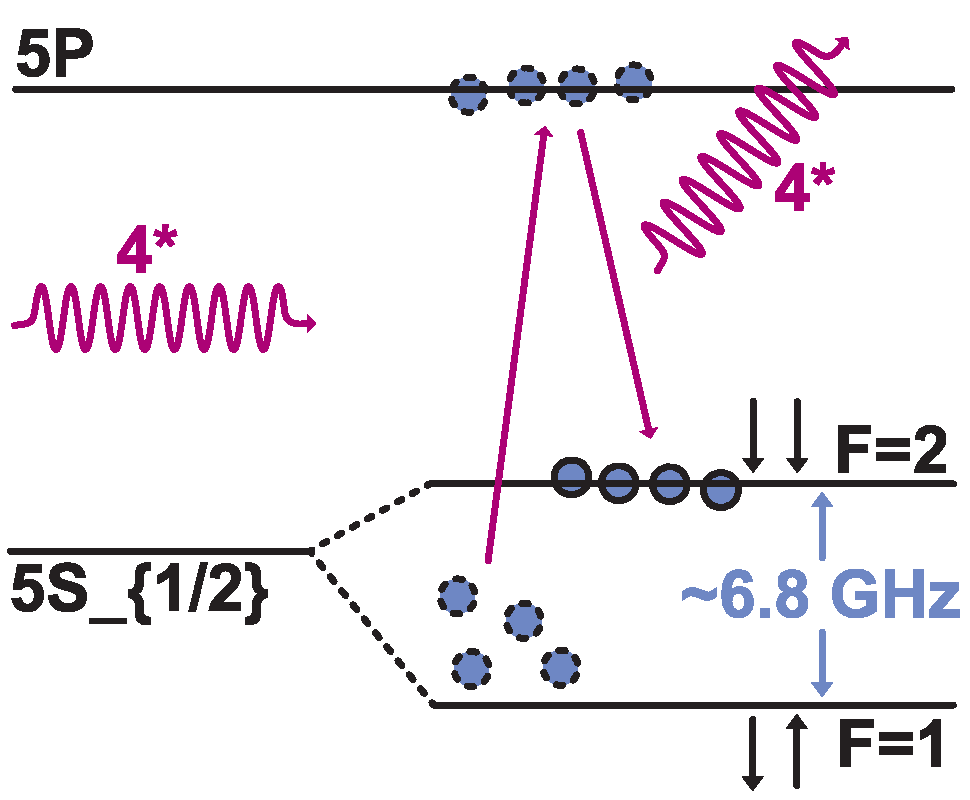
\includegraphics[width=\linewidth]{pdf/MODR/pumping-decay.pdf}
        \caption{Population inversion and decay.}
        \label{fig:MODR-pumping-decay}
    \end{minipage}
    %
    \hfill
    %
    \begin{minipage}[t]{0.3\linewidth}
        \centering
        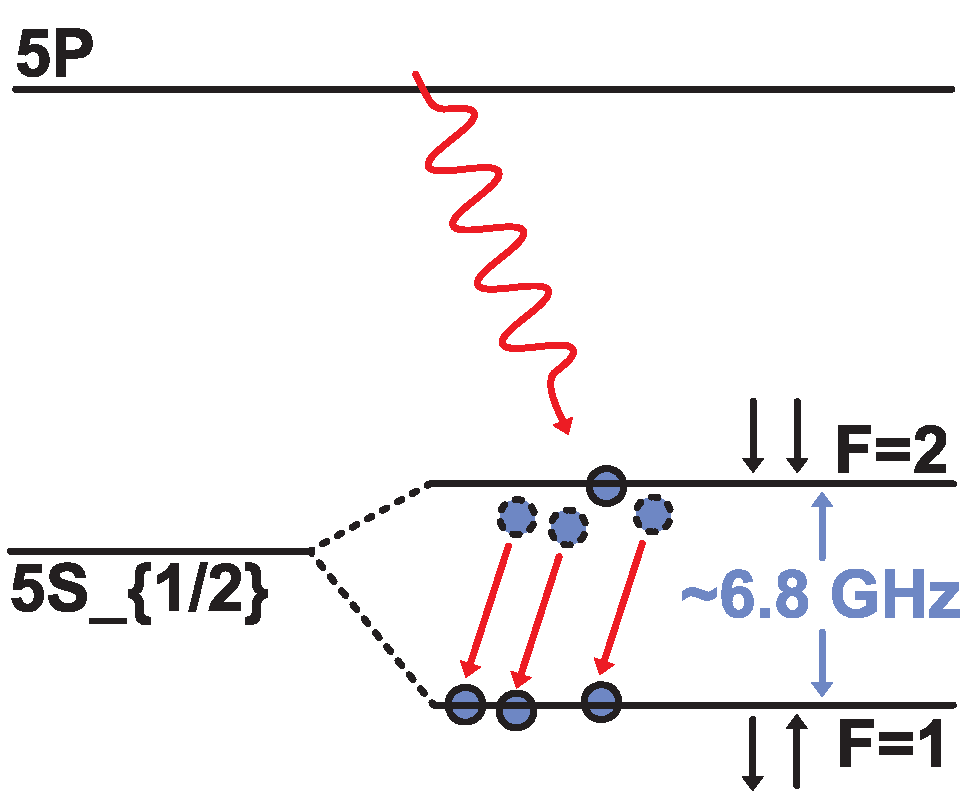
\includegraphics[width=\linewidth]{pdf/MODR/microwave.pdf}
        \caption{Microwave excitation.}
        \label{fig:MODR-microwave}
    \end{minipage}
    %
    \hfill
    %
    \begin{minipage}[t]{0.3\linewidth}
        \centering
        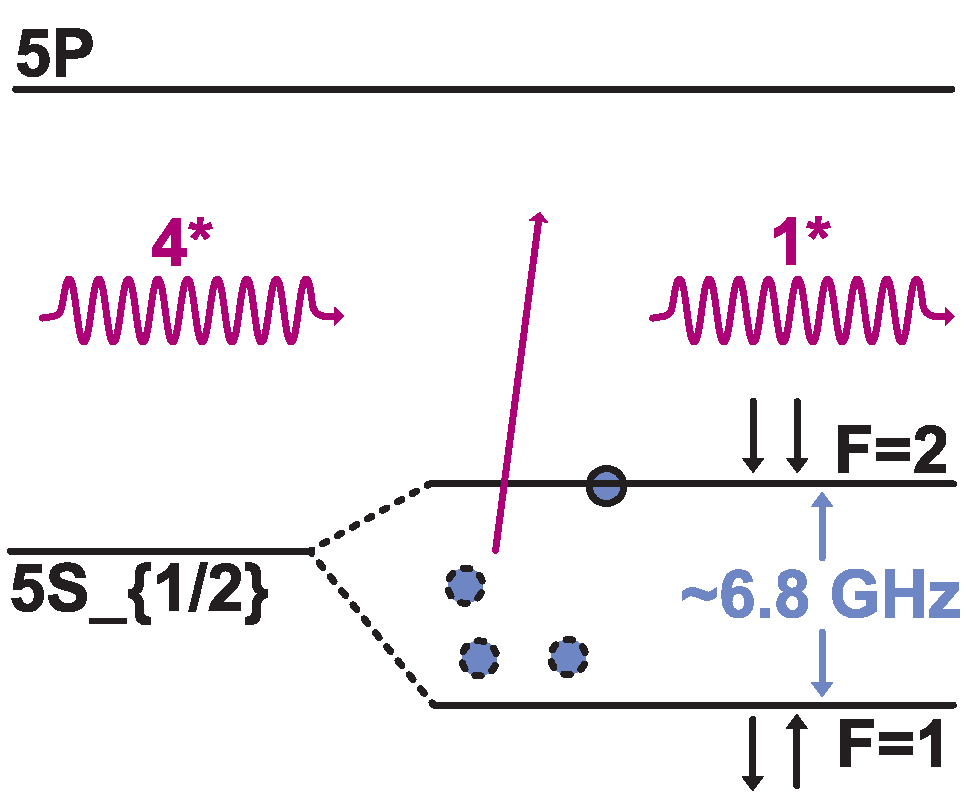
\includegraphics[width=\linewidth]{pdf/MODR/interrogation.pdf}
        \caption{Optical interrogation.}
        \label{fig:MODR-interrogation}
    \end{minipage}

    \caption{Electrons cycle in a MODR-based \acrshort{csac} due to the optical pumping, microwave excitation, and optical interrogation.}
    \label{fig:MODR-steps}
\end{figure}

With reference to Figure \ref{fig:MODR-steps}, we can now analyze deeper the different stages of the cycle and understand how it's possible to detect whether the microwave signal is in resonance with the atomic transition or not.

In particular, in Figure \ref{fig:MODR-pumping-decay} we can see four high energy photons coming from the pumping source that excite the electrons found at $5S_{1/2} F=1$, to $5^2P_{1/2}$ state.
From here, electrons will decay to both the $5^2S_{1/2} F=2$ and the $5^2S_{1/2} F=1$ states.
Over time however, the population will tend to accumulate on the $5^2P_{1/2} F=2$ state given that the excitation photons are not coupled with the \ref{itm:Rb-III} transition (due to the filter cell action).

During the second stage (Figure \ref{fig:MODR-microwave} for reference), the microwave excitation coming from the local oscillator is used to force the decay of the electrons from the $5^2S_{1/2} F=2$ state to the $5^2S_{1/2} F=1$ state.
Notice, however, that the decay is possible only if the microwave signal is at the right frequency of the transition, that is \ref{itm:Rb-I}.
In case the microwave signal is not exactly in resonance with the atomic transition, not all the electrons will be forced to decay and some of them will remain in the excited state.
Figure \ref{fig:MODR-microwave} shows an example where the microwave signal is not in perfect resonance with the atomic transition and 1 out of the 4 electrons remain in the $5^2S_{1/2} F=2$ state.

Finally, the cycle is closed with the interrogation phase (Figure \ref{fig:MODR-interrogation}).
Here, by sending the same amount of irradiation as in the pumping phase, we are able to detect if electrons are in the $5^2S_{1/2} F=1$ state or in the $5^2S_{1/2} F=2$ state.
In particular, in case not the entire population has decayed to the $5^2S_{1/2} F=1$ state during the microwave excitation, the interrogation phase will show a different intensity of the transmitted light.
In Figure \ref{fig:MODR-interrogation}, we can see that 1 out of the 4 photons will be transmitted given that only 3 atoms are in the $5^2S_{1/2} F=1$ state.

By measuring the intensity of the transmitted light, we can understand if the microwave signal was in resonance with the atomic transition or not.


\paragraph{Photodetector}

At the end of the vapor gas cell, a photodetector is used to measure the intensity of light transmitted through the reference cell.

In case of a MODR-based \acrshort{csac}, only if the microwave signal was in resonance with the atomic transition, most of the laser source from the bulb lamp will be absorbed by the atoms and the transmitted light will be minimal.
Conversely, in case of a non-resonant microwave signal, the intensity of the transmitted light will be stronger.

The signal captured by the photodetector is then sent to the control loop that will use it to fine-tune the local oscillator frequency.
